\documentclass[11pt, a4paper]{report}

\usepackage{graphicx}
\graphicspath{ {images/} }

\usepackage{hyperref}
\usepackage[xindy]{glossaries}
\makeglossaries
\makeindex

\usepackage[utf8]{inputenc}
\usepackage{csquotes}

\usepackage[square,sort,comma,numbers]{natbib}
\bibliographystyle{IEEEtran}

\usepackage{amsmath}
\newcommand\addtag{\refstepcounter{equation}\tag{\theequation}}
\usepackage{txfonts}

\setlength{\parindent}{0ex}
\setlength{\parskip}{1ex}

\begin{document}
\begin{titlepage}
    \title{IP6 - Report Street Networks}
    \date{\today}
    \author{J. Peyer, S. Merki}
    \maketitle
\end{titlepage}
\setcounter{page}{1}

\tableofcontents



\begin{abstract}
    Text here.
\end{abstract}

\chapter{Introduction}

\chapter{Theoretical Task}
\section{Shape Grammar}
The main key of shape grammar is to generate networks and paintings by a new defined grammar based on shape rules, selection rules, painting rules and limiting shapes. Shape grammar is a language based on an alphabet of shapes and generated shapes. Like the authors G. Stiny and J. Gips describe in "Shape Grammars and the Generative Specification of Painting and Sculpture  \citep{shapeGrammars:1972}.
\begin{displayquote}
    Definition. A shape grammar (SG) is a 4-tuple: $SG = (V_T, V_M, R, I)$ where
    \begin{enumerate}
        \item $V_T$ is a finite set of shapes.
        \item $V_M$ is a finite set of shapes such that $V_T $* $\cap$  $V_M = \emptyset$
        \item R is a finite set of ordered pairs (u.v) such that u is a shape consisting of an element of $V_T $* combined with an element of $V_M$ and v is a shape consisting of (A) the element of $V_T $* contained in u or (B) the element of $V_T $* contained in u combined with an element of $V_M$ or (C) the element of $V_T $* contained in u with an additional element of $V_T$* and an element of $V_M$.
        \item I is a shape consisting of elements of $V_T $* and $V_M$.
    \end{enumerate}
\end{displayquote}
The following image describes the generative specifications and some examples rules.
\pagebreak
\begin{displayquote}
\begin{figure}[!h]
    \centering
        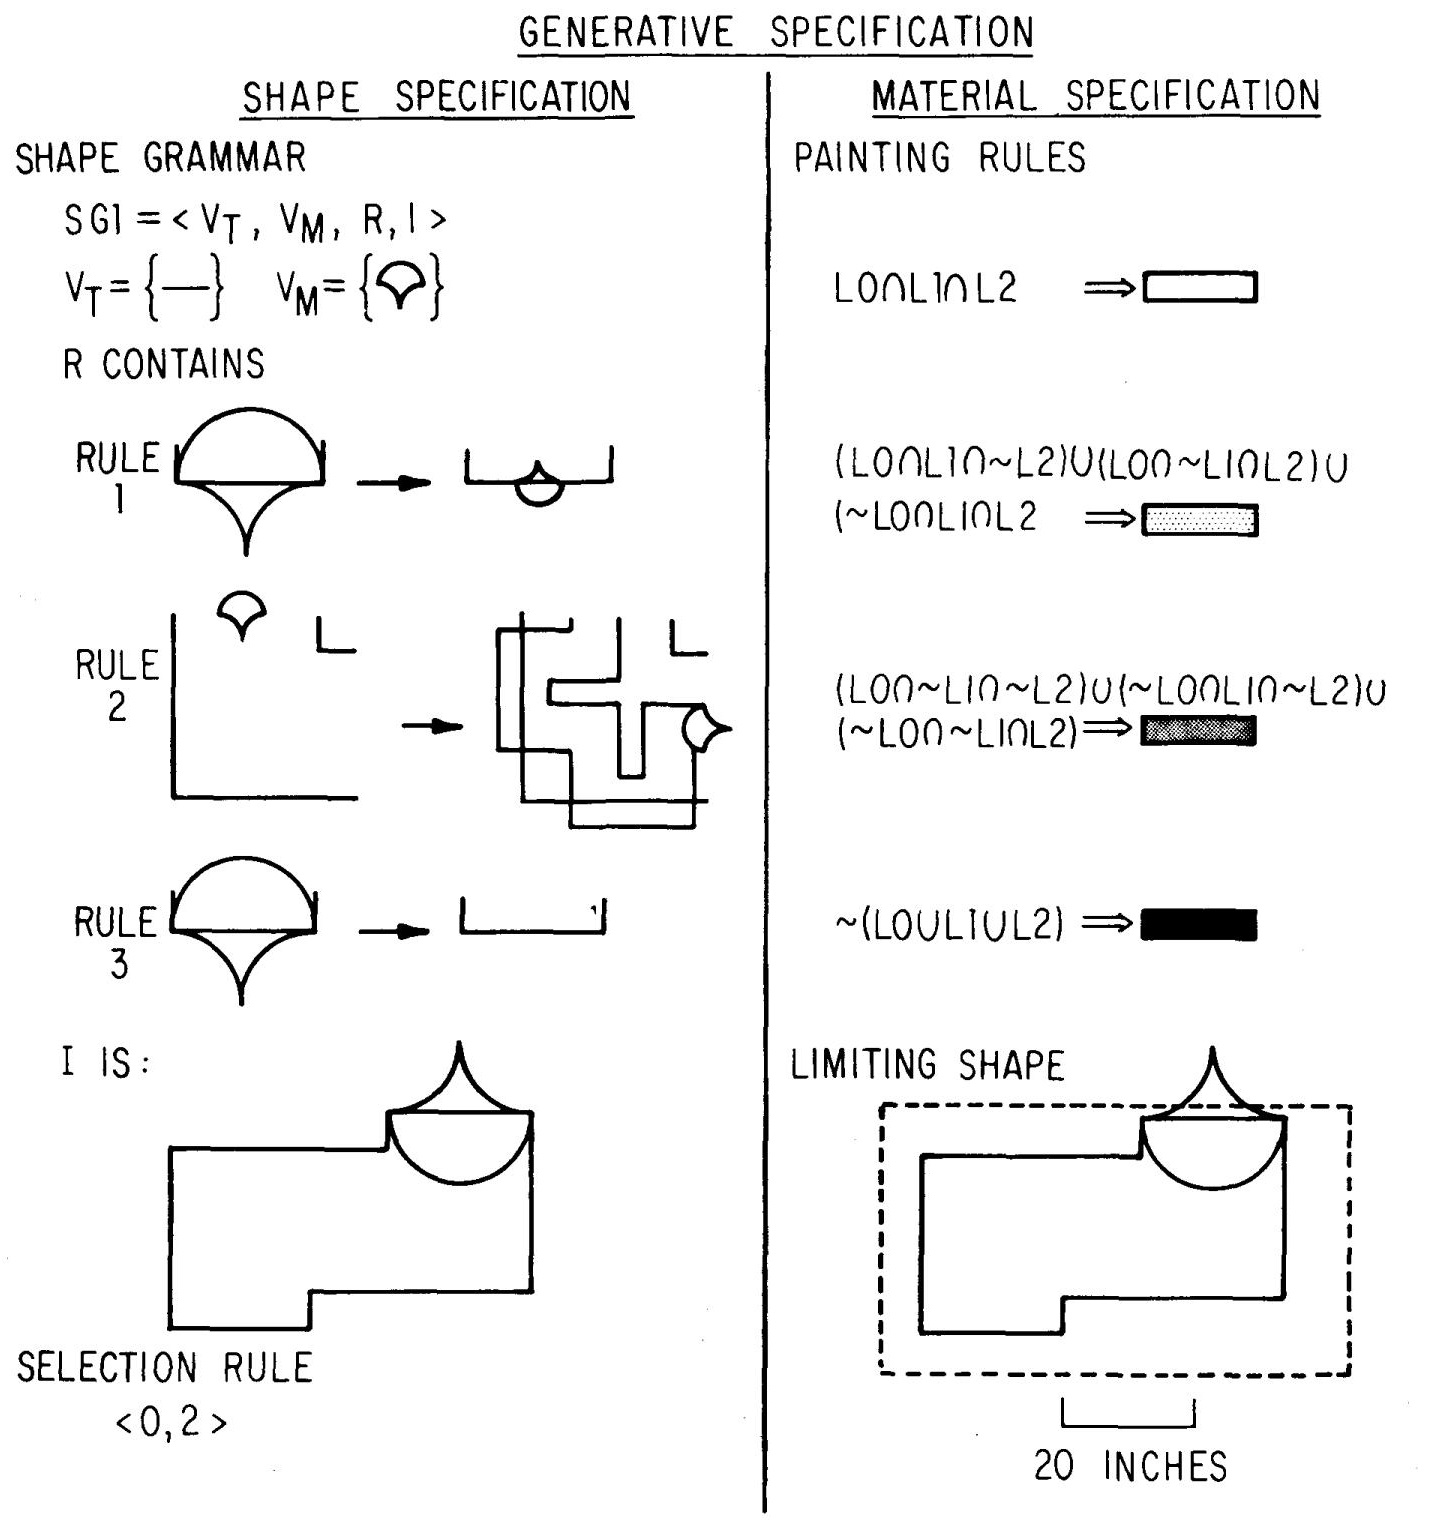
\includegraphics{generativ_specification}
    \caption{ Complete, generative specification of the class of  paintings con-
        taining Urform I, II,  and  III. \citep{shapeGrammars:1972}}
\end{figure}
\end{displayquote}

\subsection{Shape Rules}
A shape rule is de definition what should be painted based on the current state of the painting. The Initial Shape has not to be inside of the Limiting Shapes.

\pagebreak
\subsection{Selection Rules}
An undefined count of shape rules provide the generation of the painting. Therefore a mechanism to select a correct shape is required. The depth is defined by levels. Like the authors G. Stiny and J. Gips describe in "Shape Grammars and the Generative Specification of Painting and Sculpture  \citep{shapeGrammars:1972}.
\begin{displayquote}
    Level assignments are made to terminals during the generation of a shape using these rules:
    \begin{enumerate}
        \item The terminals in the initial shape are assigned level 0.
        \item If a shape rule is applied, and the highest level assigned to any part ot the terminal corresponding to the level side of the rule is N, then
        \begin{enumerate}
            \item If the rule is of type A, any part of the terminal enclosed by the marker in the left side of the rule is assigned N.
            \item If the rule is of type B, any part of the terminal enclosed by the marker in the left side of the rule is assigned N and any part of the terminal enclosed by the marker is assigned N + 1.
            \item If the rule is of type C, the terminal added is assigned N + 1.
        \end{enumerate}
        \item No other level assignments are made.
    \end{enumerate}
\end{displayquote}

\subsection{Painting Rules}
Painting rules describe witch shape should be painted inside of a defined area. Like in a Venn diagram the rules contain multiple levels 0 - n. By combining this levels the painting colour is described. As describes in more details by the authors G. Stiny and J. Gips in "Shape Grammars and the Generative Specification of Painting and Sculpture \citep{shapeGrammars:1972}.
\begin{displayquote}
    Painting rules indicate how the areas contained in a shape painted by considering the shape as a Venn diagram as in naive set theory. The terminals of each level in a shape are taken as the outline of a set in the Venn diagram. As parts ot terminals may be assigned multiple levels, sets may have common boundaries. Levels 0, 1, 2, ..., n are said to define sets L0, L1, L2, ..., Ln respectively where n is given in the selection rule.
    \newline
    A painting rule has two sides separated by a double arrow ($\Rightarrow$). The left side of a painting rule defines a set using the sets determined by level assignment and the usual set operators, for example, union($\bigcap$), intersection ($\bigcup$), complementation($\sim$), and exclusive or ($\bigotimes$), The sets defined by the left side of the painting rules of M must partition the universal set. The right side of a painting rule is a rectangle painted in the manner the set defined by the left side of the rule is to be painted.
\end{displayquote}

\subsection{Limiting Shapes}
These Shapes define a limiting area on the canvas, where shape painting is allowed. 
The area could have any form, but normally it is defined as a rectangle. Like a camera view the Limiting Shape define the scale of a painting and its viewpoint. Therefore the initial/start shape could be outside of the limiting shape 

\subsection{Sculpture}

\subsection{Aesthetics}

\pagebreak
\section{Procedural Modelling}

\pagebreak
\section{L-Systems}

L-System is a well established modelling approach for the synthesis of realistic plant images. There are many papers describing L-Systems and how they are applied to generate plant live: [TODO: reference those papers] "In these cases L-System productions capture the \textit{development} of plant components over time." \citep{PrusinkiewiczEtAl:2001} Productions are applied in parallel, so that all plant parts grow and age equally. The growth is stopped at a defined terminal age. This age is the number of iterations, where in each iteration productions are applied.
\subsection{TODO: reference papers here}
The context-free productions in \citep{PrusinkiewiczEtAl:2001} are defined using the following syntax.
\[
pred : \{block1\}\ cond\ \{block2\} \leadsto succ \addtag
\]
The symbol \textit{pred} (predecessor) defines the module that will get replaced by the modules defined in \textit{succ} (successor). This replacement is only applied, if the (optional) condition is met. \textit{block1} and \textit{block2} are C statement blocks, of which the first block is executed before and the second after the condition is evaluated.
\subsection{Notes JP}

\pagebreak
\section{Chomsky Grammars?}
\citep{PrusinkiewiczEtAl:2001}
Almost like L-System but with minor modifications.

\pagebreak
\chapter{Practical Task}
\section{CPlan}
\subsection{Changes}
\begin{itemize}
    \item The function .toArray() creates a complete copy of the existing enumeration in the ram. Therefore the application had an extremely large footprint. To reduce the coping we changed some methods to be called directly with IEnumerable Parameters.
    \item If some extension methods are created the should be tested by unit tests.
\end{itemize}


\subsection{New Functions}
\subsubsection{Graph to Tree}


\chapter{Conclusion}

\bibliography{quotations}
\appendix
\glsaddall
\printglossaries
\end{document}